\documentclass[12pt,a4paper,openany]{ctexrep}
%ctexrep:报告格式,可用chapter,part,默认封面、目录自动分页。
%ctexbook:书籍格式,同上,奇偶页左右边距不同。
%ctexart:文章格式,不可用chapter,part,封面,目录同正文同一页。

%===================标题信息
\def \title {市场综合管理信息服务平台\\\, \\技术方案}
\def \author {作者}
\def \department {部门名称}
\def \custom	{信阳金牛大别山农产品现代物流中心}
\def \company {郑州闪创网络科技有限公司}
\def \Ecompany {Zhengzhou Lighting Creative Technology Co.,Ltd}

%===================调用宏集
\usepackage{lettrine}				%首字下沉

\usepackage{graphicx}				

\usepackage{geometry}		

\usepackage{multirow}				%表格纵向合并

\usepackage{makeidx}				%索引
\makeindex							%启动索引功能

\usepackage{array}

\usepackage{hyperref}				%引用书签

\usepackage{longtable}			%跨页表单

%===================文档从这里开始
\geometry{left=3cm,right=3cm,top=3cm,bottom=3cm}
\begin{document}	

%===================标题部分
\thispagestyle{empty}
\begin{center}
	\parbox[t][3cm][c]{\textwidth}{\Large
	\begin{center} {{\custom}} \end{center} }
	
	\parbox[t][8cm][c]{\textwidth}{{\fontsize{32pt}{20pt}{
	\begin{center} {\textbf{\title}}\end{center} }}}
	
	\parbox[t][8cm][t]{\textwidth}{
	\begin{center}  {\large{(第一期)}}\end{center} }

	\parbox[b][2cm][c]{\textwidth}{ {\large
	\begin{center}
	\company \\
	\Ecompany 
	\end{center}}}
	
	\parbox[b][2cm][b]{\textwidth}{
	\begin{center} {\large\textbf{\number\year \,·\,\number\month}} \end{center} }
\end{center}

%===================目录部分
\newpage
\setcounter{page}{1}
\pagenumbering{Roman}				%页码以罗马数字计数
\tableofcontents					%生成目录

%===================正文部分
%===================章节
\chapter{项目总体功能概述及建设总路线图}
%\setcounter{page}{1}				%重置页码(注意位置,要在\chapter行下边
\pagenumbering{arabic}			%页码以阿拉伯数字表示
\lettrine[lines=2]{本}\, 方案在原架构方案基础上,结合金牛大别山农产品现代物流中心实际需求紧迫度及建设周期,提出整体平台的功能模块划分,各期建设规划。市场综合管理信息服务平台计划共分六期建设,依次是\textbf{市场及商户管理模块},\textbf{仓储管理及监控模块},\textbf{市场交易信息收集模块},\textbf{市场财务管理系统},\textbf{市场线上B2B商城},\textbf{冷链物流管理模块}。\par

\begin{description}
\item[第一期\, 市场及商户管理模块]主要完成市场的商铺管理,常驻商户信息管理;实现商户线上缴纳租金,费用自动统计及定期生成报表;市场内部通知公告。\par
\item[第二期\, 仓储管理及监控模块]主要完成市场纯人工平库的数字化货物管理,并将现阶段使用中的自动、半自动化仓库的数据统一进行抽出汇总,在此基础上完成后台对所有类别仓库的信息查看,定向查询。在仓库内设置多点位视频探头及温控探头,并通过数据接口实现管理后台对于仓库的实时监控,实现异常温度自动报警。\par
\item[第三期\, 市场交易信息收集模块]主要完成市场内交易货物的采样及统计功能。本模块通过商户主动货物申报,车辆扫牌识别,地磅等软硬件联动,并结合仓库出入库货物信息,实现市场内车辆管理、吞吐货物量估算、客流量统计。
\item[第四期\, 市场财务管理模块]主要完成市场财务相关管理,包括日常记账,账户管理,固定资产管理,期末结转,损益结算,财务报表,报税,银企直联,日常报销等。
\item[第五期\, 市场线上B2B商城]主要完成市场线上B2B商城建设,通过供、需两方面建立市场上下游供应链,建立线上商品统筹配送,并对接物流企业完成自动发货,逐步开拓线上零售市场。
\item[第六期\, 冷链物流管理模块]主要完成市场供应链建设过程中的运输,仓储监控功能,配合市场线上商城以及作为市场后续发展方向的冷链物流业务。
\end{description}

本项目由郑州闪创网络科技有限公司提供全程项目技术研发,软硬件接口对接\footnote{部分已有软硬件设备接口需要市场方对接之前的开发方提供}以及项目的\hyperref[arrange]{部署实施},\hyperref[arrange]{员工培训},技术维护。

本方案着重介绍第一期建设及实施路线图。第一期建设内容如表~\ref{function}所示:

\begin{table}[htbp]
\begin{tabular*}{\hsize}{p{3cm}<{\centering}|p{3cm}<{\centering}|p{8cm}}
\hline
模块划分					&	平台				&	\multicolumn{1}{c}{主要功能}		\\
\hline
市场前端(第一期)		&	PC网站,公众号		&	市场信息,商户登录,商户信息,缴纳租金,系统通知		\\
\hline
市场管理后台(第一期)	&	PC网站				&	商户信息,商铺信息,租金管理,发布通知,缴费信息统计及报表		\\	
\hline
\end{tabular*}
\caption{项目一期建设功能模块}
\label{function}
\end{table}

通过项目第一期建设,主要解决现阶段市场在商铺租金管理,商户信息统计上管理较为粗放的问题,
\begin{itemize}
\item 一可以为市场管理者提供市场商户、商铺的实时直观化信息;
\item 二可以促进市场内商户租金定期缴纳,防止偷费漏费;
\item 三可以将PC网站及公众号作为市场线上门户,逐步通过线上开展业务宣传及业务推广。
\end{itemize}

%===================章节
\chapter{市场PC网站功能模块(第一期)}
\lettrine[lines=2]{市}\, 场PC网站主要包括【首页(市场信息)】、【商户展示】、【商户中心】、【消息中心】。本PC网站金牛大别山农产品物流中心的门户网站,用于介绍市场,商户销售产品等信息展示。同时本网站也作为商户中心的入口,用户登录之后可以查看市场商铺空位,租金价格,成为商户后可以进行线上租金缴纳,查看市场通知。在后续平台建设过程中会逐步增加线上商城、仓储管理、信息统计等功能。\par

\section{首页(市场信息)}
\begin{description}
\item[宣传banner]市场或商户的宣传banner图,可以放置多张轮播,可以跳转店铺链接或第三方网站;
\item[市场介绍]金牛大别山农产品物流中心介绍图文,包括市场简介,发展历程,合作商家,主营业务等;
\item[联系我们]市场联系方式,位置等信息。
\end{description}

\section{商户展示}
\begin{description}
\item[商户列表]以列表形式,按商品大类展示已经入驻本市场的商户信息。包括商户名称,\hyperref[main_business]{商品大类},主营商品,店铺位置,店主姓名,联系方式,\hyperref[shop_cover]{店铺展示照片};
\item[店铺详情页]点击店铺卡片进入店铺详情页,展示以上字段,以及\hyperref[shop_cover]{店铺照片、商品照片};
\item[查找商户]用户可以通过商户名称,商品大类,主营商品进行查找。
\end{description}

\section{商户中心}
\subsection{用户登录}
\begin{description}
\item[手机号登录]输入手机号,发送验证码,输入正确的验证码进行登录;
\item[微信登录]微信扫码进行登录,若未绑定手机号需要先绑定手机号再进行微信扫码登录;
\item[支付宝登录]支付宝扫码进行登录,若未绑定手机号需要先绑定手机号再进行扫码登录;
\item[QQ登录]QQ扫码进行登录。
\end{description}

\subsection{查看商铺}
\begin{description}
\item[我的商铺列表]商铺编号、商铺租金、租金支付方式(月付/季付/年付)、商铺租期、签约时间、商铺到期时间、交租日期、合同附件;
\item[市场商铺信息]商铺编号、商铺租金、租金支付方式(月付/季付/年付)、是否出租、租期、租赁合同模板、申请。
商铺信息可以选择【列表】或【视图】方式显示。通过【视图】可以以3D视图的形式直观化看到现在市场内各商铺信息及租用情况。
\item[申请商铺预约]填写需要申请的商铺编号,申请人信息,开始时间,并提交后台审核。审核通过后后台可以将申请表格打印好,申请的商户直接前往市场信息管理中心签字盖章,快速办理入驻申请。
\end{description}

\subsection{缴纳租金}
\begin{description}
\item[缴纳租金]以月为单位按期缴纳,一次缴纳多个月的租金可以通过后台设置折扣优惠。
\item[缴费记录]缴费金额、支付月份、缴费时间、支付方式(支付宝/微信/线下转账)、备注信息。
\end{description}

\subsection{编辑商户信息}
\begin{description}
\item[商户经营者信息]店主姓名,联系方式,自动读取店铺在市场内的位置信息;
\item[店铺照片]可以上传店铺照片和商品照片。上传照片时选择类别【店铺照片】,【商品照片】。可以将某张照片设为展示用照片\label{shop_cover}。
\item[主营商品]店铺商品大类,店内主要销售的具体商品\label{main_business};
\item[绑定车牌号]本店常用车牌号码,用于三期开发时数据调用。
\end{description}

\section{消息中心}
PC网站的新消息会以红点的形式在网站的消息中心图标上显示,并显示具体的未读条数。消息中心中的消息同时会在公众号端进行消息通知提示,参见\hyperref[3.3]{3.3\, 消息推送}。项目第一期中,消息中心内容包含市场发布的通知公告,及系统自动生成的租金,入驻申请等方面的消息提示。
\begin{description}
\item[市场通知]显示市场管理方发给各店铺店主的消息通知,例如表~\ref{ex1};

\begin{table}[htbp]
\begin{center}
\begin{tabular}{|p{10cm}|}
\hline
\centerline{\large{市场春节期间营业时间公告}}\\
尊敬的店主:\\
本市场在春节期间正常营业,请各店铺根据自身实际情况安排营业时间。\\
\vspace{0cm}
金牛大别山农产品物流中心\quad 运营部\\
\hline
\end{tabular}
\end{center}
\caption{市场春节期间营业时间公告}
\label{ex1}
\end{table}

\item[系统消息]显示各类线上申请,服务,提示等系统自动生成的消息。例如表~\ref{ex2}。

\begin{table}[htbp]
\begin{center}
\begin{tabular}{|p{10cm}|}
\hline
尊敬的店主:\\
您的店铺(编号0123456)租期将于2020年5月1日结束,请您及时通过线上或前往市场信息管理中心进行交付。租金逾期后每日将按照月租金5‰额外征收滞纳金。\\
\hline
\end{tabular}
\end{center}
\caption{租金到期提示消息}
\label{ex2}
\end{table}

\end{description}

%===================章节
\chapter{市场公众号建设(第一期)}
\section{市场信息}
\subsection{市场介绍}
在微信后台编辑好自动回复模板,用户点击后自动推送市场简介信息。

\subsection{商户信息}
点击进入商户信息H5页面。
\begin{description}
\item[商户列表]以列表形式,按商品大类展示已经入驻本市场的商户信息。包括商户名称,\hyperref[main_business]{商品大类},主营商品,店铺位置,店主姓名,联系方式,\hyperref[shop_cover]{店铺展示照片};
\item[店铺详情页]点击店铺卡片进入店铺详情页,展示以上字段,以及\hyperref[shop_cover]{店铺照片、商品照片};
\item[查找商户]用户可以通过商户名称,商品大类,主营商品进行查找。
\end{description}

\section{商户中心}
\subsection{我的商铺}
点击进入我的商铺H5页面。
\begin{description}
\item[我的商铺列表]商铺编号、商铺租金、租金支付方式(月付/季付/年付)、商铺租期、签约时间、商铺到期时间、交租日期、合同附件;
\item[市场商铺列表]商铺编号、商铺租金、租金支付方式(月付/季付/年付)、是否出租、租期、租赁合同模板、申请。
\item[申请商铺预约]填写需要申请的商铺编号,申请人信息,开始时间,并提交后台审核。审核通过后后台可以将申请表格打印好,申请的商户直接前往市场信息管理中心签字盖章,快速办理入驻申请。
\end{description}

\subsection{缴纳租金}
点击进入缴纳租金H5页面。
\begin{description}
\item[缴纳租金]以月为单位按期缴纳,一次缴纳多个月的租金可以通过后台设置折扣优惠。
\item[缴费记录]缴费金额、支付月份、缴费时间、支付方式(支付宝/微信/线下转账)、备注信息。
\end{description}

\begin{figure}[htbp]
\centering
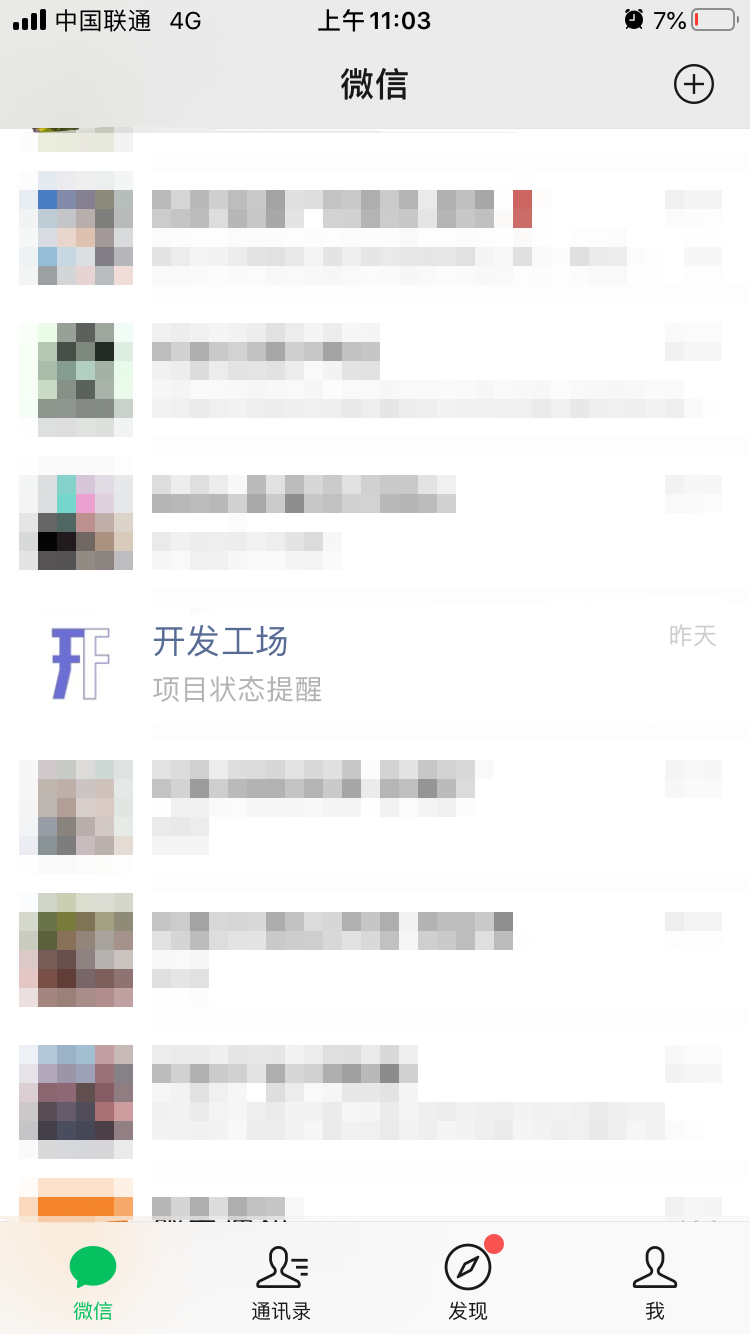
\includegraphics[width=6cm]{fig/wechat1.png}\qquad \qquad
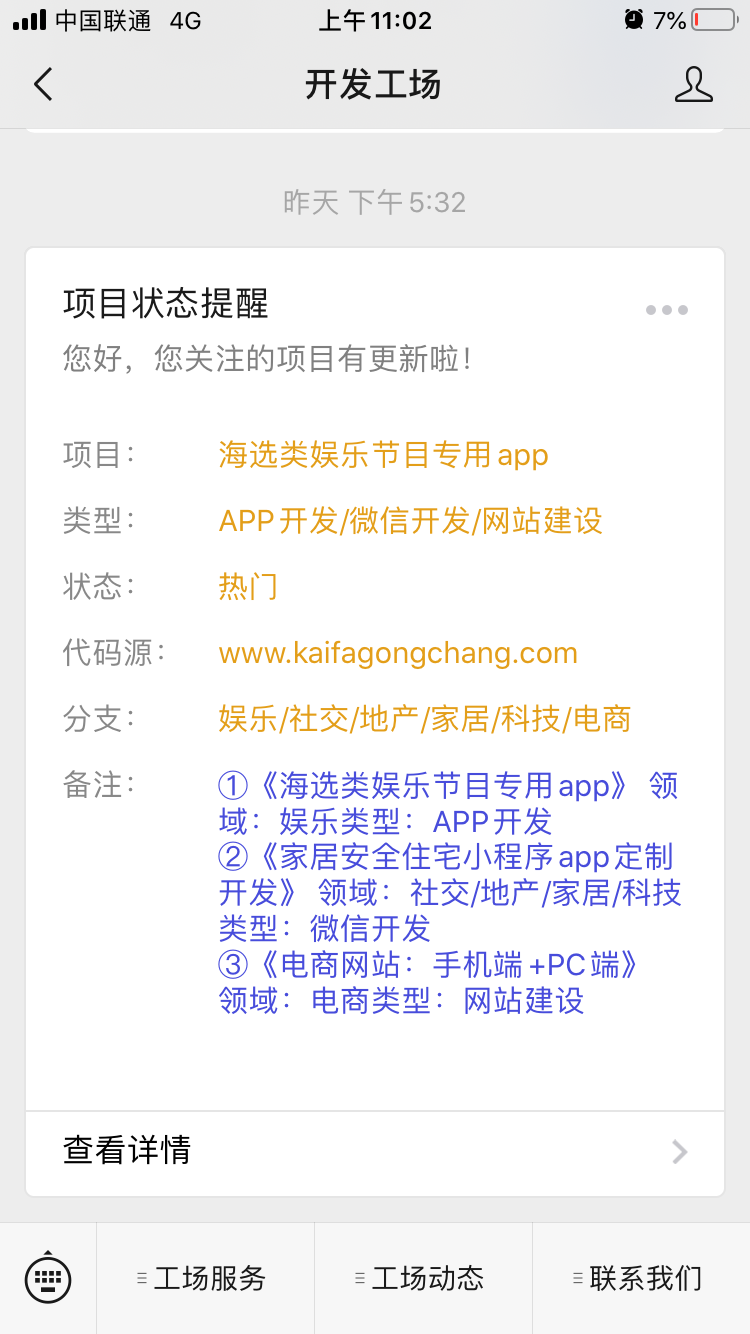
\includegraphics[width=6cm]{fig/wechat2.png}
\caption{微信消息通知}
\label{wechat_message}
\end{figure}

\subsection{个人设置}
点击进入个人设置H5页面。
\begin{description}
\item[商户经营者信息]店主姓名,联系方式,自动读取店铺在市场内的位置信息;
\item[店铺照片]可以上传店铺照片和商品照片。上传照片时选择类别【店铺照片】,【商品照片】。可以将某张照片设为展示用照片\label{shop_cover}。
\item[主营商品]店铺商品大类,店内主要销售的具体商品\label{main_business};
\item[绑定车牌号]本店常用车牌号码,用于三期开发时数据调用。
\end{description}

\section{消息推送}
\label{3.3}
公众号消息推送采用消息卡片形式进行。每当有新消息时,会在公众号形成消息卡片,并通过微信公众号APP进行消息提示。
样式如图~\ref{wechat_message}所示。

\begin{description}
\item[市场通知]显示市场管理方发给各店铺店主的消息通知;
\item[系统消息]显示各类线上申请,服务,提示等系统自动生成的消息。
\end{description}

%===================章节
\chapter{市场管理后台(第一期)}  
\section{首页}
建立市场3D视图,管理员可以通过3D视图的形式直观化看到现在市场内各商铺信息及租用情况。

\section{商户档案}
查看入驻商户信息,包括店主信息,主营产品,绑定车牌信息,平台账号ID,所在店铺,租金缴费情况,历史数据等。\\
※平台账号和商户账号不是同一个账号,商户账号需通过后台创建,可以关联到平台账号。
\begin{description}
\item[新建商户]店主姓名,身份证号,身份证照片正反面,联系手机号码,住址,租赁商铺(可多个),平台账号ID;
\item[查看商户]根据区域,店主姓名,商铺编号,手机号,是否欠费等筛选。
\end{description}

\section{商铺档案}
包括商铺编号、商铺面积、商铺租金、所在大区。管理人员可以创建新商铺或编辑现有商铺信息。
\begin{description}
\item[新建商铺]商铺编号、商铺面积、所在大区、商铺租金、租金支付方式(月付/季付/年付);
\item[租赁中商铺]商铺编号、商铺面积、所在大区、商铺租金、租金支付方式(月付/季付/年付)、商铺租期、签约时间、商铺到期时间、交租日期、合同附件、缴费记录、租赁人员信息\footnote{店主信息,主营产品,绑定车牌信息,平台账号ID等};
\item[租赁统计]根据月份筛选,新签数量、租约金额、已支付金额、待支付金额。
\end{description}

\section{发布通知}
\begin{description}
\item[消息通知]显示已发送的通知标题、介、发布时间、发布区域,图文详情;
\item[新建消息]消息标题、消息简介、图文详情。新消息可以按品类大区发布。
\end{description}

\section{banner图管理}
\begin{description}
\item[banner列表]显示banner图预览,顺序,跳转链接;
\item[新建banner]上传新图片,设置顺序,跳转链接。
\end{description}

%===================章节
\chapter{项目预期进度}
\lettrine[lines=2]{本}\, 项目第一期预计五月上旬开始进行原型设计,后续计划如表~\ref{schedule}所示。在项目推进过程中,于原型设计完成及UI设计完成后会同市场方进行确认,市场方对于原型功能及UI设计风格没有异议之后进行项目技术研发。本项目预计工期为20个工作日。
\begin{table}[htbp]
\begin{tabular*}{\hsize}{p{2.5cm}<{\centering}@{-}p{2.5cm}<{\centering}|p{7cm}|p{3cm}}
\hline
\multicolumn{2}{c|}{时间节点}		&	进度内容				&	备注	\\
\hline
\multicolumn{2}{c|}{五月上旬}		&	项目立案,需求整理,原型设计		&			\\
\multicolumn{2}{c|}{五月中旬}		&	UI设计								&			\\
五月下旬		&		六月上旬		&	技术开发							&			\\
\multicolumn{2}{c|}{六月中旬}		&	项目测试,试运行,项目优化		&			\\
\multicolumn{2}{c|}{六月下旬}		&	项目正式运行						&			\\
\hline
\end{tabular*}
\caption{项目预期建设进度}
\label{schedule}
\end{table}

%===================章节
\chapter{项目部署实施}
\label{arrange}
\lettrine[lines=2]{本}\, 项目由闪创科技负责全程部署实施,主要包括:【项目试运行及优化】,【软件部署】,【市场相关业务人员培训】。

\section{项目试运行及优化}
本项目在开发过程中采用通用标准及功能进行开发,同时考虑到市场方的具体操作习惯及优化市场商户用户体验,本项目开发阶段分为【开发及测试】,【试运行及优化】两个阶段进行。\par
\begin{description}
\item[开发及测试]本项目由闪创科技进行全程技术研发,开发完成后由闪创科技负责完成项目的内部测试,保证项目可以完成本需求文档及原型内所提出的功能需求;
\item[试运行及优化]项目开发及测试完成后,由闪创科技责成专人技术小组入驻金牛大别山农产品物流中心,负责项目的试运行及优化工作。在试运行期间,闪创科技技术小组在已经研发完成的项目基础上针对市场管理方使用人员的操作体验、操作习惯,完成优化工作。同时在市场内随机选择愿意参与测试的商户进行商户的操作及体验度优化。
\end{description}

\section{软件部署}
软件部署主要包括服务器端\footnote{服务器可采用市场现有服务器,如现有服务器不能满足功能需求,则需另行采购}环境及数据库部署及PC端程序部署。\par
闪创科技负责项目开发及测试完成后的项目部署工作。在服务器端包括整体运行语言环境的搭建,数据库环境搭建。\par
在PC端主要包括项目可用的浏览器安装,市场各管理人员账号创建及权限设置。\par

\section{市场相关业务人员培训}
闪创科技负责本项目的操作培训工作。\par
项目开发及测试完成后,由闪创科技责成专人对市场内所有使用本项目的业务人员进行针对性培训,包括该业务人员使用的前端页面功能操作,bug及突发情况处置方式等内容。

\section{运维及售后服务}
\subsection{项目运维支持服务}
本项目从项目规划设计到实施落地全部由专项项目成员负责,对于后期项目运维支持由专业的团队负责。
\begin{itemize}
\item 按照市场的统一要求,成立市场管理系统项目建设的专项团队,有序开展研发工作;
\item 根据新的工作方式,确定相关人员的岗位职责,实现业务处理由线下到线上的平稳过渡;
\item 双方建立联合工作团队,落实好各自的职责,确保项目按期保质保量完成.
\end{itemize}

\subsection{项目售后服务}
闪创科技对于产品售后服务非常全面,后续可根据业务变化进行相关功能产品进行适应性的调整,实现信息化产品全过程管理。运维人员会维护上线运行的全部模块。维护内容包含系统故障类服务、系统优化类服务、日常运维类服务、巡视检查类服务、专项保障类服务。
\begin{description}
\item[系统故障类服务]针对用户在使用过程中遇到的软硬件环境问题、系统管理、系统bug、系统配置问题等提供优质的服务;
\item[系统优化类服务]根据具体事件内容,闪创科技会派遣专业人员为用户制定详细的调优方案;
\item[日常运维类服务]为用户的日常运维提供快速响应服务、现场服务、远程服务等几类日常运维服务;
\item[巡视检查类服务]实施及试运行期间会有专项团队负责按周对应用系统进行例行检查,系统交付完毕后根据双方签署的服务协议提供系统检查服务。
\item[专项保障类服务]闪创科技提供“安全保障、灾难恢复”等专项保障类服务,可以对用户的数据安全性、系用户的数据安全性、系统安全性提供保障。统安全性提供保障。
\end{description}
\paragraph{}

%===================附录部分
\appendix							%附录部分以\appendix开始,后续同正文样式

\chapter{第一期所需数据表单及接口}
\lettrine[lines=2]{为}\, 了减少开发过程中出现的对接问题,以下为在原型设计及开发过程中所需要的各类表单信息及技术接口。支付宝、微信、腾讯等接口申请请参见帮助文档,如果需要闪创科技协助申请,请市场方事先联系\footnote{在接口申请过程中可能需要市场方提供市场法人身份证信息,代理办理人手机、身份证等信息,如果市场方有保密上的顾虑,可以参考说明文档自行申请。}。
所需各类表单及接口如表~\ref{interface}所示。
\begin{longtable}{p{3.5cm}|p{6cm}|p{4.5cm}}
\hline
\multicolumn{1}{c|}{表单及接口名称}		&	\multicolumn{1}{c|}{说明}		&	\multicolumn{1}{c}{备注}		\\
\hline
市场入驻申请信息	&	商户在入驻本市场时需要提交的信息,例如商户姓名,业务范围等	&	用于制作线上预约入驻服务申请表单	\\
\hline
商铺信息			&	每个门面包含的信息,例如位置,面积,租金等						&	用于设计商铺管理模块		\\	
\hline
市场商品大类列表	&	例如干果一区、水果二区、蔬菜一区之类的市场现在大区分类的名称		&	用于制作市场虚拟结构		\\
\hline
市场信息			&	例如市场简介,地理位置,发展历程,联系方式,负责人,负责人简介等		&	用于制作市场网站首页		\\
\hline
市场宣传照片		&	市场各类环境照片,员工工作照,商户工作照,市场logo等			&	用于设计市场网站首页		\\	
\hline
市场服务器配置表	&	市场现有服务器配置表												&	用于评估是否需要购买新服务器		\\
\hline
支付宝商户平台账号	&	支付宝支付接口\footnotemark[1],免费申请					&	用于支付宝登录	\\
\hline
微信公众平台账号	&	微信公众平台\footnotemark[3],免费申请							&	用于微信公众号开发及部署		\\	
\hline
微信开放平台账号	&	微信公众平台\footnotemark[4],免费申请							&	用于微信登录	\\
\hline
腾讯开放平台账号	&	腾讯开放平台\footnotemark[5],免费申请							&	用于qq登录		\\
\hline
龙支付账号			&	建行龙支付账号														&	用于租金缴费等支付	\\
\hline
\caption{表单及接口列表}
\label{interface}
\end{longtable}
\footnotetext[1]{支付宝,知托付 \url{https://www.alipay.com/}}
\footnotetext[3]{微信公众平台 \url{https://mp.weixin.qq.com/}}
\footnotetext[4]{微信开放平台 \url{https://open.weixin.qq.com/}}
\footnotetext[5]{微信开放平台 \url{https://open.qq.com/mobi_guide/}}

\chapter{项目软硬件技术参数参考}
本项目参考软硬件配置参数如表~\ref{server},表~\ref{software}所示。
\begin{table}[htbp]
\begin{longtable}{p{3cm}|p{9.5cm}|p{1.5cm}}
\hline
\multicolumn{1}{c|}{类别}		&	\multicolumn{1}{c|}{参数}		&		\multicolumn{1}{c}{数量}\\
\hline
服务器主机		&	多后端服务器,确保业务安全及可用性;采用集群模式部署;linux 8核+16G+300GSSD	&	2台	\\
\hline
数据库服务器	&	高性能数据库服务器,确保业务高可用性;linux 8核+16G+200GSSD	&	2台\\	
\hline
redis服务器	&	数据持久化机制确保数据备份可靠,提供数据持久化。Linux 8核+16G+200GSSD	&	1台		\\
\hline
SSL证书			&	HTTPS传输加密协议,为客户端(浏览器) 到服务器端之间搭建一条加密通道,保证数据在传输过程中不被窃取或篡改,确保机密信息的保密性、完整性和可信性	&	1个\\
\hline
\caption{服务器参考参数}
\label{server}
\end{longtable}
\end{table}

\begin{table}[htbp]
\begin{longtable}{p{3cm}|p{9.5cm}|p{1.5cm}}
\hline
\multicolumn{1}{c|}{类别}	&	\multicolumn{1}{c|}{参数}	&	\multicolumn{1}{c}{备注}\\
\hline
开发语言		&	java1.8								&	\\
\hline
数据库			&	支持mysql5.8、sql server2008		&	\\	
\hline
运行环境		&	tomcat8								&	\\
\hline
\caption{软件参考参数}
\label{software}
\end{longtable}
\end{table}

%===================参考文献部分
%\begin{thebibliography}{*}		%*缺省
%\bibitem{bib1} sth.,sth.,sth.,sth.
%\end{thebibliography}

%===================索引部分
%\printindex						%输出索引,输出前需先进行编译“MakeIndex”

\end{document}